\section{Operations of the Computer Hardware}
\begin{frame}{Operations of the Computer Hardware}
\begin{figure}\caption{Arithmatic Instructions in MIPS}
\begin{center}
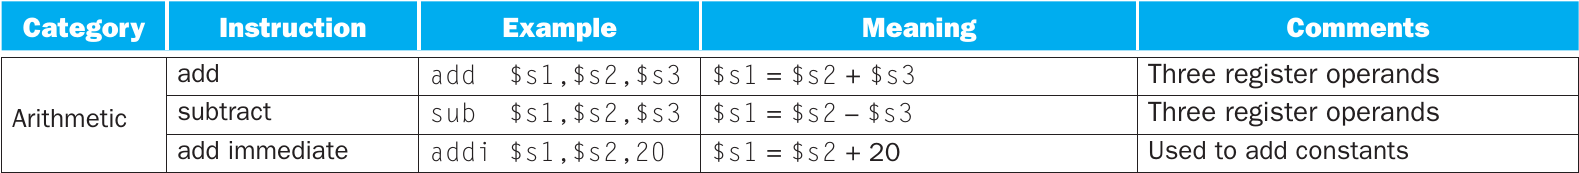
\includegraphics[width=\textwidth, height=0.2\textheight]{docs/images/operations-1}
\end{center}
\end{figure}
\end{frame}

\begin{frame}{Operations of the Computer Hardware (Cont'd)}
\begin{table}[H]
\begin{adjustbox}{width=\textwidth}
\begin{tabular}{|c|c|c|c|}
\hline
load word & \texttt{lw \$s1, 20(\$s2)} & \texttt{\$s1 = Memory[\$s2 + 20]} & Word from memory to register \\
\hline
store word & \texttt{sw \$s1, 20(\$s2)} & \texttt{Memory[\$s2 + 20] = \$s1} & Word from register to memory \\
\hline
load byte & \texttt{lb \$s1, 20(\$s2)} & \texttt{\$s1 = Memory[\$s2 + 20]} & Byte from memory to register \\
\hline
load byte unsigned & \texttt{lbu \$s1, 20(\$s2)} & \texttt{\$s1 = Memory[\$s2 + 20]} & Byte from memory to register \\
\hline
store byte & \texttt{sb \$s1, 20(\$s2)} & \texttt{Memory[\$s2 + 20] = \$s1} & Byte from register to memory \\
\hline
load upper immed & \texttt{lui \$s1, 20} & \texttt{\$s1 = 20 * $2^{16}$} & Loads constant in upper 16 bits \\
\hline
\end{tabular}
\end{adjustbox}
\caption{Data Transfer Instructions in MIPS}
\end{table}
\end{frame}

\begin{frame}{Operations of the Computer Hardware (Cont'd)}
\begin{figure}\caption{Logical Instructions in MIPS}
\begin{center}
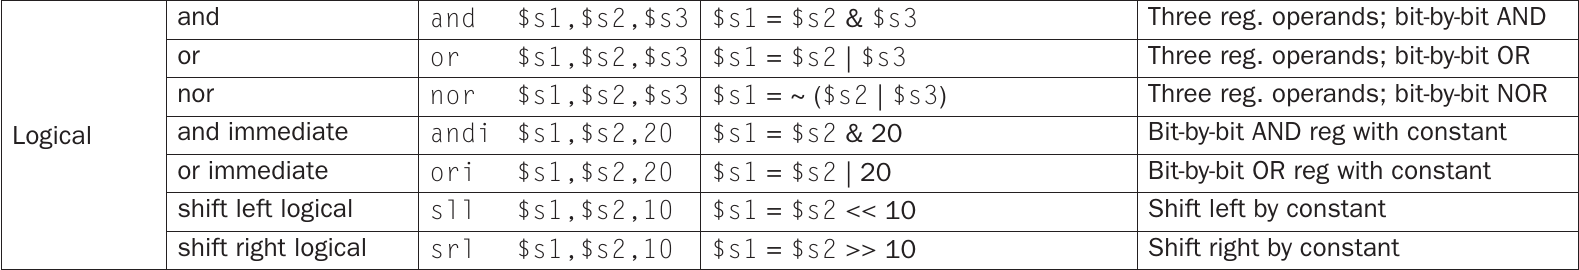
\includegraphics[width=\textwidth, height=0.4\textheight]{docs/images/operations-3}
\end{center}
\end{figure}
\end{frame}

\begin{frame}{Operations of the Computer Hardware (Cont'd)}
\begin{figure}\caption{Conditional Branch Instructions in MIPS}
\begin{center}
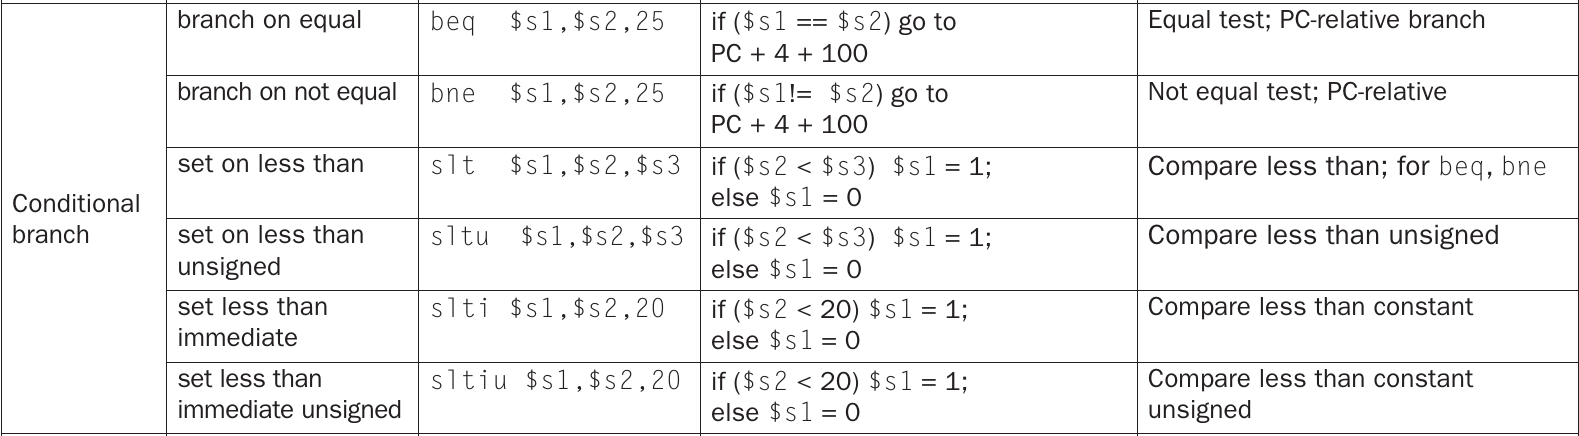
\includegraphics[width=\textwidth, height=0.5\textheight]{docs/images/operations-4}
\end{center}
\end{figure}
\end{frame}

\begin{frame}{Operations of the Computer Hardware (Cont'd)}
\begin{figure}\caption{Unconditional Jump Instructions in MIPS}
\begin{center}
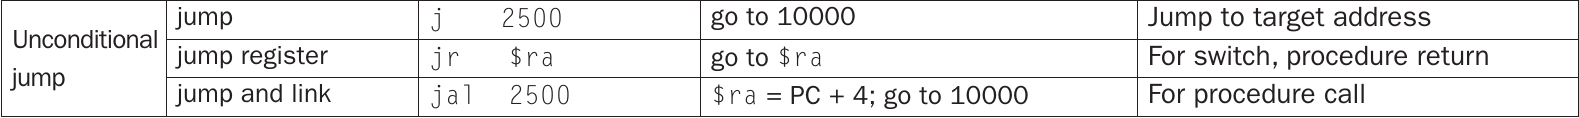
\includegraphics[width=\textwidth, height=0.17\textheight]{docs/images/operations-5  }
\end{center}
\end{figure}
\end{frame}

\begin{frame}{Example - Compiling a Complex C Assignment into MIPS}
\begin{flushleft}
A somewhat complex statement contains the five variables \texttt{f}, \texttt{g}, \texttt{h}, \texttt{i}, and \texttt{j}:

\hspace{8mm}\texttt{f = (g + h) – (i + j);}

What might a C compiler produce?
\end{flushleft}
\end{frame}

\begin{frame}[fragile]{Answer}
\begin{itemize}
\item[-]
\texttt{add t0, g, h \# temporary variable t0 contains g + h}

\item[-]
\texttt{add t1, i, j \# temporary variable t1 contains i + j}

\item[-]
\texttt{sub f, t0, t1 \# f gets t0 – t1, which is (g + h) – (i + j)}
\end{itemize}
\end{frame}

\section{Operands of the Computer Hardware}
\begin{frame}{Example - Compiling a C Assignment Using Registers}
\begin{flushleft}
It is the compiler’s job to associate program variables with registers. 

Take, for instance, the assignment statement from our earlier example:

\hspace{8mm}\texttt{f = (g + h) – (i + j);}

The variables \texttt{f}, \texttt{g}, \texttt{h}, \texttt{i}, and \texttt{j} are assigned to the registers \texttt{\$s0}, \texttt{\$s1}, \texttt{\$s2}, \texttt{\$s3},
and \texttt{\$s4}, respectively. 

What is the compiled MIPS code?
\end{flushleft}
\end{frame}

\begin{frame}[fragile]{Answer}
\begin{itemize}
\item[-]
\texttt{add \$t0, \$s1, \$s2  \# register \$t0 contains g + h}

\item[-]
\texttt{add \$t1, \$s3, \$s4  \# register \$t1 contains i + j}

\item[-]
\texttt{sub \$s0, \$t0, \$t1  \# f gets \$t0 – \$t1, which is (g + h) – (i + j)}
\end{itemize}
\end{frame}

\subsubsection{Memory Operands}
\begin{frame}{Example - Compiling Using Load and Store}
\begin{flushleft}
Assume variable \texttt{h} is associated with register \texttt{\$s2} and the base address of the array \texttt{A} is in \texttt{\$s3}. 

What is the MIPS assembly code for the C assignment state­
ment below?

\hspace{8mm}\texttt{A[12] = h + A[8];}
\end{flushleft}
\end{frame}

\begin{frame}{Answer}
\begin{itemize}
\item[-]
\texttt{lw \$t0, 32(\$s3) \# Temporary reg \$t0 gets A[8]}

\item[-]
\texttt{add \$t0, \$s2, \$t0  \# Temporary reg \$t0 gets h + A[8]}

\item[-]
\texttt{sw \$t0, 48(\$s3)  \# Stores h + A[8] back into A[12]}
\end{itemize}    
\end{frame}

\subsubsection{Constant or Immedidate Operands}
\begin{frame}{Constant or Immedidate Operands}
\begin{itemize}
\item[-] \texttt{addi \$s3, \$s3, 4  $\, \, \, \, \,$ \# \$s3 = \$s3 + 4}
\end{itemize}
\end{frame}

\section{Representing Instructions}
\begin{frame}{Instructions Big Picture}
\begin{table}[H]
\begin{adjustbox}{width=\textwidth}
\begin{tabular}{|c|c|c|c|c|c|c|c|c|}
\hline
Name & Format & \multicolumn{6}{|c|}{Example} & Comments \\
\hline
\hline
Field Size && 6 bit & 5 bit & 5 bit & 5 bit & 5 bit & 6 bit & All MIPS instructions are 32 bits long \\
\hline
R-format & R & op & rs & rt & rd & shamt & funct & Arithmetic instruction format \\
\hline
\texttt{add} & R & 0 & 18 & 19 & 17 & 0 & 32 & add \texttt{\$s1,\$s2,\$s3} \\
\hline
I-format & I & op & rs & rt & \multicolumn{3}{|c|}{address} & Data transfer format\\
\hline
\texttt{lw} & I & 35 & 18 & 17 & \multicolumn{3}{|c|}{100} & lw \texttt{\$s1,100(\$s2)} \\
\hline
J-format & J & op & \multicolumn{5}{|c|}{address} & Unconditional Branch \\
\hline
\texttt{j} & J & 8 & \multicolumn{5}{|c|}{300} & jump to address \\
\hline
\end{tabular}
\end{adjustbox}
\end{table}
\end{frame}

\section{Logical Operations}
\begin{frame}{Logical Operations Big Picture}
\begin{figure}
\begin{center}
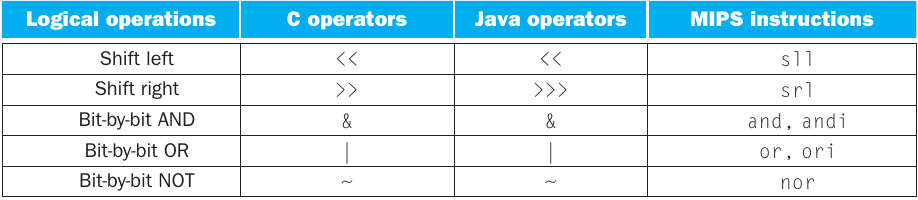
\includegraphics[width=\textwidth, height=0.4\textheight]{docs/images/logical}
\end{center}
\end{figure}
\end{frame}

\section{Instuctions for Making Decisions}
\begin{frame}{Instructions for Making Decisions}
\begin{itemize}
\item[-]
\texttt{beq register1, register2, L1}

This instruction means go to the statement labeled \texttt{L1} if the value in \texttt{register1}
equals the value in \texttt{register2}.

The mnemonic beq stands for \textit{branch if equal}.

\vspace{5mm}
\item[-]
\texttt{bne register1, register2, L1}

It means go to the statement labeled \texttt{L1} if the value in \texttt{register1} does not equal
the value in \texttt{register2}.

The mnemonic \texttt{bne} stands for \textit{branch if not equal}.
\end{itemize}
\end{frame}

\begin{frame}[fragile]{Example - Compiling \textit{if-then-else} into Conditional Branches}
\begin{flushleft}
In the following code segment, \texttt{f}, \texttt{g}, \texttt{h}, \texttt{i}, and \texttt{j} are variables. 

If the five variables, \texttt{f} through \texttt{j}, correspond to the five registers \texttt{\$s0} through \texttt{\$s4}, what is the
compiled MIPS code for this C if statement?

\begin{lstlisting}[language=python, keywordstyle=\color{purple}\textbf]
if i == j:
    f = g + h
else:
    f = g – h
\end{lstlisting}
\end{flushleft}
\end{frame}

\begin{frame}[fragile]{Answer}
\begin{lstlisting}[keywords={bne, add, j, sub}, keywordstyle=\color{purple}\textbf]
bne $s3, $s4, Else       # go to Else if i != j
add $s0, $s1, $s2        # f = g + h (skipped if i != j)
j   Exit                 # go to Exit
Else: 
    sub $s0, $s1, $s2    # f = g – h (skipped if i = j)
Exit:
\end{lstlisting}    
\end{frame}

\begin{frame}[fragile]{Example - Compiling a \textit{while} Loop in C}
\begin{flushleft}
Here is a traditional loop in C:
\begin{lstlisting}[language=c, keywordstyle=\color{purple}\textbf]
while (save[i] == k){
    i += 1;
}
\end{lstlisting}

Assume that \texttt{i} and \texttt{k} correspond to registers \texttt{\$s3} and \texttt{\$s5} and the base of the
array \texttt{save} is in \texttt{\$s6}.

What is the MIPS assembly code corresponding to this
C segment?
\end{flushleft}
\end{frame}

\begin{frame}[fragile]{Answer}
\begin{lstlisting}[keywords={sll, add, lw, bne, addi, j}, keywordstyle=\color{purple}\textbf]
Loop:   sll     $t1,$s3,2       # Temp reg $t1 = i * 4
        add     $t1,$t1,$s6     # $t1 = address of save[i]
        lw      $t0,0($t1)      # Temp reg $t0 = save[i]
        bne     $t0,$s5, Exit   # go to Exit if save[i] != k
        addi    $s3,$s3,1       # i = i + 1
        j       Loop            # go to Loop
Exit:
\end{lstlisting}
\end{frame}

\section{Suporting Precedures in Computer Hardware}
\begin{frame}{Six Steps}
\begin{enumerate}
\item Put parameters in a place where the procedure can access them.
\item Transfer control to the procedure.
\item Acquire the storage resources needed for the procedure. 
\item Perform the desired task.
\item Put the result value in a place where the calling program can access it. 
\item Return control to the point of origin, since a procedure can be called from several points in a program.
\end{enumerate}
\end{frame}

\begin{frame}{Provided Registers}
\begin{flushleft}
MIPS software follows the following convention for procedure calling in allocating its 32 registers
\end{flushleft}

\begin{itemize}
\item[-]
\texttt{\$a0-\$a3}: four argument registers in which to pass parameters
\item[-] \texttt{\$v0-\$v1}: two value registers in which to return values
\item[-] \texttt{\$ra}: one return address register to return to the point of origin    
\end{itemize}
\end{frame}

\begin{frame}{Provided Registers (Cont'd)}
\begin{itemize}
\item[-] In addition to allocating these registers, MIPS assembly language includes an instruction just for the procedures: 

\item[-]\textit{It jumps to an address and simultaneously saves the address of the following instruction in register \texttt{\$ra}.} 

\item[-]The \textit{jump-and-link} instruction (\texttt{jal}) is simply written:

\item[-] \texttt{jal ProcedureAddress}
\end{itemize}
\end{frame}

\begin{frame}{Provided Registers (Cont'd)}
\begin{itemize}
\item[-] 
The \textit{link} portion of the name means that an address or link is formed that points to
the calling site to allow the procedure to return to the proper address. This ``link",
stored in register \$ra (register 31), is called the return address. 

\item[-] The return address
is needed because the same procedure could be called from several parts of the
program.

\item[-]To support such situations, computers like MIPS use jump register instruction
(\texttt{jr}), introduced above to help with case statements, meaning an unconditional
jump to the address specified in a register:

\item[-] \texttt{jr \$ra}
\end{itemize}
\end{frame}
\section{MIPS Addressing for 32-Bit Immediates and Addresses}
\section{A C Sort Example to Put It All Together}